\section{Model with noise and discretization}

There are several sources of noise in a micro-bolometer setup:
\begin{itemize}
\item Thermal noise in the resistances,
\item Flicker noise in resistances,
\item Burst noise,
\item Thermal fluctuations in the bolometer temperature,
\item Noise in incident IR radiation,
\item Noise in read out circuits.
\end{itemize}

In this report we shall only consider the first two types of noises,
thermal and flicker noise in resistances.

\subsection{Thermal noise}

Any resistance with a temperature $T$ above zero, will cause the
charge carriers in the material to fluctuate. The fluctuations are
independent of each other, and will generate a current with a
voltage. This phenomenon is referred to as thermal noise, but is also
known as white noise and Johnson noise. This type of noise was first
discovered by the Swedish engineer John
B. Johnson~\cite{PhysRev.32.97}, and his colleague Harry Nyquist, also
Swedish, provided a theory for the noise based on statistical
physics\cite{PhysRev.32.110}. One of the characteristics of the noise,
is the flat power spectrum for all most all frequencies, which is also
characteristic for white light.

In electrical circuits, thermal noise is commonly modeled as an additional
power source in series with the resistance, see Figure~\ref{fig:johnsonEquivalentNoise}.
\begin{figure}
  \centering
  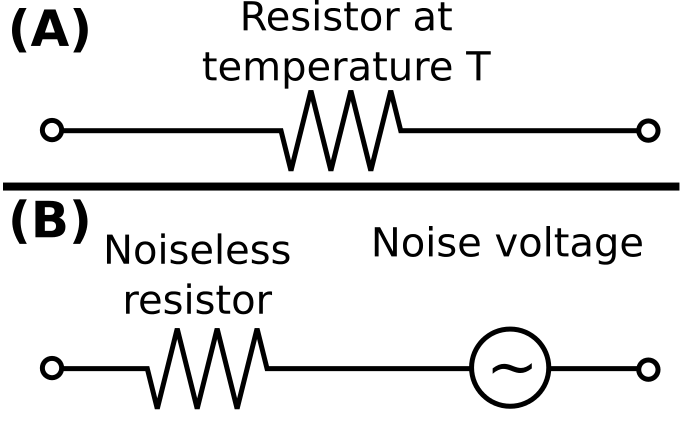
\includegraphics[width=0.5\textwidth]{gfx/JohnsonNoiseEquivalentCircuits.png}
  \caption{Equivalent model for thermal noise in a resistor.}~\label{fig:johnsonEquivalentNoise}
\end{figure}
Due to the random nature of the additional power source, it is not
possible to predict the instantaneous voltage produced, but instead the
average behavior. Nyquist\cite{PhysRev.32.110} found that the power
spectrum of thermal noise to be
\begin{equation}
  \label{eq:power_spectrum_white_noise}
  S(f) = 4 k_B T R,
\end{equation}
where $k_B$ is the Boltzmann constant, $T$ is the temperature of the
resistance, and $R$ is the resistance. The total contribution of the
noise source is then calculated by summing up the contribution from
each frequency component.
\begin{equation}
  \label{eq:2}
  \E \left[ V^2 \right] = \int_B S(f) \mathrm(d) f,
\end{equation}
where $B$ is the bandwidth of the circuit.

% The mean square square voltage o

A statistical model commonly used to white noise is a stationary stochastic
process where the auto-correlation function is
\begin{equation}
  \label{eq:autocorrelation_white_noise}
  R(s,t)={\frac {\operatorname {E} [(X_{t}-\mu _{t})(X_{s}-\mu
      _{s})]}{\sigma _{t}\sigma _{s}}} =
  \begin{cases}
    \sigma_{t}^2 , \quad t = s, \\
    0 , \quad t \neq s
  \end{cases}
\end{equation}
meaning that the process is uncorrelated in time. A distribution that
can be used for this process is the Gaussian distribution
$\mathcal{N}(0, \sigma)$.

\subsection{Flicker Noise}\label{sec:flicker-noise}

Another type of noise source that exists in circuits is flicker
noise, or also known as low frequency noise, 1/$f$ noise or pink noise. The power
spectrum of the Flicker noise is
\begin{equation}
  \label{eq:power_spectrum_flicker_noise}
  S(f) \propto \frac{k}{f^{\alpha}}.
\end{equation}
where $\alpha \in [0.5, 1.5]$ and $k$ is a material constant.

One explanation of the occurrence of the flicker noise in resistors is
that the charge carriers get trapped in capture sites of the
conductor, and are then released with variable rates. This was first
explained by Schottky for flicker noise in vacuum tubes~\cite{PhysRev.28.74}.

To generate the flicker noise in simulation there are several methods
available, listed in~\cite{381848}.

\subsection{Noise model and simulation scheme}

To compensate for the noise in the read-out circuit, one first has to
determine how noise enters the differential equation governing the
behavior of the system. The simplest possible solution is of course to
add a noise term of a normally distributed character to the left hand side
in Equation~\eqref{eq:heat_balance_equation}, rendering the theory for
diffusion processes readily available. More precisely we rewrite Equation~\eqref{eq:heat_balance_equation}
as
\begin{align} \label{eq:heat_balance_equation_noise1}
 CdT&=\left(\frac{V_b(t)^2}{R(T)}+\varepsilon(P_t+P_s -2A_s \sigma
      T^4)-G_{leg}(T-T_s)
      \right)dt + K(t)dW \\
 T(0)&=T_s	\nonumber
\end{align}
where $K$ is a function of time, and $W \sim N(0, dt)$.
The function $K(t)$ is chosen according to the following heuristic.
We expect the noise in the output to be the cause of resistor fluctuations.
Motivated by the setup for Figure~\ref{fig:johnsonEquivalentNoise}, we thus redefine the voltage over
the bolometer resistance as
\begin{equation}
  \label{eq:randomvariable_transformation}
  V \rightarrow V_0 + \Delta V,
\end{equation}
where $V_0$ is the noise-less resistance over the voltage, and $\Delta
V$ is a random variable representing the random fluctuations in the
voltage.

We thus want noise to enter the heat equation in Equation~\eqref{eq:heat_balance_equation}
roughly as
\begin{equation}
  \label{eq:heat_balance_equation_noise}
  C\frac{dT}{dt}=\frac{(V_b(t) + \Delta V)^2}{R(T)}+ f(T),
\end{equation}
where $\Delta V$ is the added noise term, accounting for the
fluctuations in the resistance $R(T)$ and $f(T)$ are the other terms
in Equation~\eqref{eq:heat_balance_equation}.
Expanding the square we get the equation
\begin{equation}
  \label{eq:heat_balance_equation_noise_SDE1}
  C\frac{dT}{dt}=\frac{1}{R(T)} (V_b^2(t) + 2 V_b(t) \Delta V + (\Delta V)^2) + f(T),
\end{equation}
If the squared noise term is negligible in the limit, we are left with
\begin{equation}
  \label{eq:heat_balance_equation_noise_SDE2}
  C\frac{dT}{dt}=\frac{1}{R(T)} (V_b^2(t) + 2 V_b(t) \Delta V  ) + f(T)
\end{equation}
Thus we chose $K(t)$ in Equation~\eqref{eq:heat_balance_equation_noise1}
as $K(t) = 2 V_b(t) \sigma$, where $\sigma$ is a parameter to be calibrated or
physically motivated. The noisy heat development can now be simulated
in a well defined setting, with the dynamics independent of step size $\Delta t$:

\begin{align} \label{eq:heat_balance_equation_noise_discr}
 CT_{i+1}&=\left(\frac{V_b(t_{i})^2}{R(T_{i})}+\varepsilon(P_t+P_s -2A_s \sigma T_i^4)-G_{leg}(T_i-T_s)\right)\Delta t + 2 V_b(t_i) \sigma \sqrt{\Delta t} W_i \\
 T(0)&=T_s	\nonumber
\end{align}

where $W_i \sim N(0,1)$.


%%% Local Variables:
%%% mode: latex
%%% TeX-master: "main"
%%% TeX-PDF-mode: 1
%%% TeX-PDF-via-dvips-ps2pdf: 1
%%% End:
